\capitulo{Revisão da literatura}
\label{cap:revisao-literatura}

Este capítulo apresenta a revisão da literatura sobre os principais conceitos que fundamentam este trabalho, abordando as tecnologias e os estudos relevantes para a análise de movimento no esporte.

\secao{Basquetebol}
\label{sec:basquete}

O basquetebol foi criado em 1891 por James Naismith, professor de Educação Física na Associação Cristã de Moços (ACM) de Springfield, Massachusetts, 
com o objetivo de desenvolver um esporte que pudesse ser praticado em ambientes fechados durante o inverno rigoroso. Segundo o Comitê Olímpico do Brasil, 
"o basquete chegou ao Brasil poucos anos depois através do americano Augusto Shaw, que em 1892 graduou-se como bacharel em Artes pela Universidade de Yale e tomou contato pela primeira vez com o basquete. 
Dois anos depois, desembarcou no Brasil para dar aulas no Colégio Mackenzie, em São Paulo. Além dos livros, trouxe também uma bola de basquete na bagagem" (COB, 2024).

As regras do basquetebol são regulamentadas pela Federação Internacional de Basquetebol (FIBA). A quadra oficial mede 28 metros de comprimento por 15 metros de largura, 
e o aro está fixado a 3,05 metros do solo. Cada equipe é composta por cinco jogadores em quadra, e o jogo é dividido em quatro períodos de 10 minutos. 
Entre as principais normas, destaca-se o tempo de posse de bola de 24 segundos e o reinício de tempo em situações específicas. Segundo as Regras Oficiais da FIBA 2020, 
“após a bola tocar o aro da cesta dos oponentes, o relógio de 24 segundos deverá ser reprogramado para: 24 segundos, se a equipe adversária obtiver o controle da bola; 
14 segundos, se a equipe que recupera o controle da bola for a mesma equipe que tinha o controle da bola antes dela tocar o aro” (CBB, 2020, p. 30).

Os fundamentos técnicos do basquetebol incluem o drible, o passe, o arremesso, o rebote e a marcação. O arremesso é considerado o fundamento mais importante, pois define a pontuação final do jogo. 
De acordo com o portal Impulsiona, ``ao conhecer o basquete, é importante ter em mente que apenas 3 movimentos são responsáveis por, talvez, mais de 80\% do tempo de jogo, criando toda a dinâmica da partida. 
Podendo ser realizados de várias formas, em separado, combinados entre si ou com outros movimentos, são eles: drible, passe e arremesso'' (IMPULSIONA, 2023).

\secao{Análise de Desempenho Esportivo}

A análise de desempenho esportivo é uma prática fundamental que visa compreender e otimizar o rendimento de atletas e equipes por meio da coleta, interpretação e aplicação de dados objetivos. 
Essa abordagem multidisciplinar envolve a avaliação de aspectos físicos, técnicos, táticos e psicológicos, permitindo uma compreensão holística do desempenho esportivo.

Segundo De Rose Júnior, Gaspar e Assumpção (2005), ``a avaliação do desempenho esportivo, por meio de diferentes indicadores (físico, técnico, tático, psicológico) de jogo, constitui-se em um método válido, objetivo e fidedigno''.

Além disso, a tecnologia tem desempenhado um papel crucial na evolução da análise de desempenho. Conforme destacado por Lamas e Morales (2022), 
``os registros de análises do desempenho nos esportes coletivos indicam extensa tradição de desenvolvimento metodológico, favorecida pela crescente disponibilidade de dados e técnicas computacionais''.

\subsecao{Análise de Desempenho no Basquetebol}

No contexto do basquetebol, a análise de desempenho tem se mostrado essencial para o desenvolvimento de estratégias e melhoria do rendimento individual e coletivo. 
A utilização de métricas específicas, como eficiência nos arremessos, número de assistências, rebotes e turnovers, proporciona uma visão detalhada das ações em quadra.

De acordo com Canan, Mendes e Silva (2015), ``arremessos de dois pontos tentados, arremessos de dois pontos convertidos, porcentagem de acerto de dois pontos, 
total de pontos feitos, porcentagem de acerto total, rebotes defensivos, rebotes totais e assistências foram considerados significativos para obtenção da vitória no jogo''.

Ferramentas como o \textit{Basketball Stats Assistant} permitem que treinadores e analistas acompanhem estatísticas em tempo real, facilitando a tomada de decisões durante as partidas. 
O aplicativo se destaca pela interface intuitiva e pelo detalhamento das estatísticas registradas durante os jogos, fornecendo uma gama ampla de funcionalidades que apoiam diretamente a análise de desempenho (Basketballstats, 2024).

Entre os principais recursos oferecidos pela ferramenta, destacam-se:

\begin{myitemize}
    \item \textbf{Registro intuitivo de ações em quadra}: permite registrar jogadas com o gesto de arrastar e soltar sobre os jogadores no campo;
    \item \textbf{Sequência de ações}: suporte a jogadas subsequentes, como rebotes ou faltas, imediatamente após a jogada principal;
    \item \textbf{Controle do tempo de jogo}: exibição do período e tempo restante, com possibilidade de edição direta no placar;
    \item \textbf{Estatísticas em tempo real}: atualizações dinâmicas sobre ações individuais e coletivas;
    \item \textbf{Correção de dados}: permite editar ou excluir eventos incorretos mesmo após a partida;
    \item \textbf{Mapas de arremesso (\textit{shot charts})}: visualização dos pontos de acerto e erro em cada área da quadra;
    \item \textbf{Estatísticas detalhadas}: coleta de dados como assistências, rebotes, roubos, faltas, tocos, turnovers, minutos jogados, entre outros;
    \item \textbf{Relatórios pós-jogo}: inclui \textit{box score}(placar), gráficos comparativos entre os jogadores ou equipes, \textit{play-by-play}, eficiência e análise de \textit{plus/minus}(Estatística usada para medir o impacto de um jogador num jogo).
\end{myitemize}


\begin{figura}{Interface do aplicativo Basketball Stats Assistant, utilizado na análise de desempenho em tempo real}{Basketball Stats Assistant (2025)}
    \begin{flushleft}
        \label{fig:app-desempenho}
        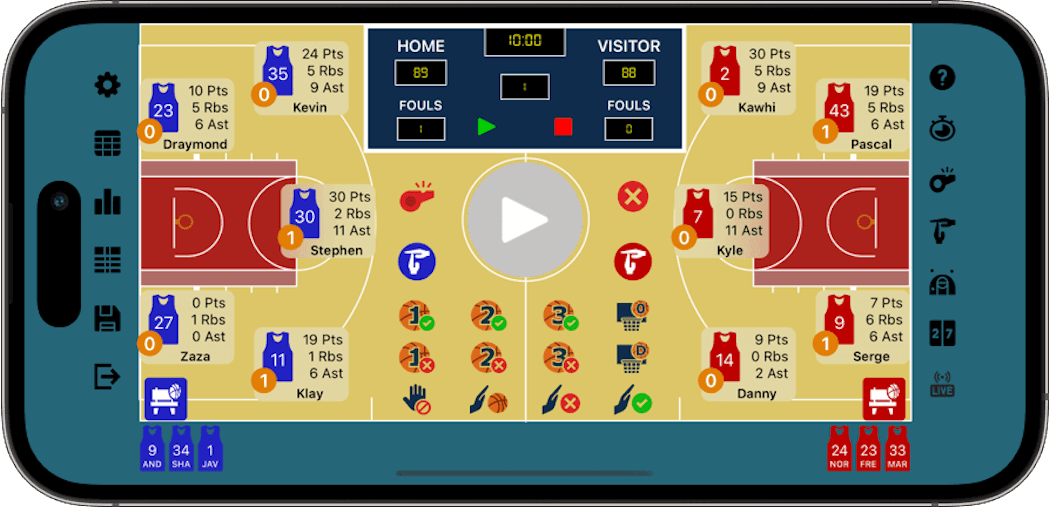
\includegraphics[width=0.7\linewidth]{resources/floats/ilustracoes/desempenho.png}
    \end{flushleft}
\end{figura}
\FloatBarrier

A análise de desempenho no basquete tem evoluído com o apoio de tecnologias como a do \textit{Basketball Stats Assistant} apresentado anteriormente, 
que permitem automatizar a coleta de métricas que auxiliam no desenvolvimento de táticas e de treinos individuais para cada tipo de atleta. 
A combinação entre dados objetivos (como distâncias percorridas e ângulos articulares) e dados estatísticos (como aproveitamento de arremessos) 
potencializa a compreensão do comportamento do atleta durante o jogo e permite intervenções mais precisas por parte da comissão técnica.

\secao{Biomecânica}

A biomecânica é a ciência que estuda os movimentos do corpo humano aplicando os princípios da mecânica. Ela busca compreender as forças internas e externas que atuam sobre o corpo e os efeitos dessas forças no desempenho atlético e na prevenção de lesões. 
Segundo Amadio e Serrão (2011), "o objetivo central da biomecânica é o estudo do movimento humano, procedendo sua análise a partir das leis da física, levando em consideração as características do aparelho locomotor" .

No contexto esportivo, a biomecânica desempenha um papel fundamental na análise e otimização dos movimentos dos atletas. Por meio da avaliação biomecânica, é possível identificar padrões de movimento inadequados, 
propor correções técnicas e desenvolver programas de treinamento personalizados, visando melhorar a eficiência e reduzir o risco de lesões. 
Brandina (2018) destaca que "a biomecânica aplicada ao esporte evidencia as estratégias usadas pelo aparelho locomotor para garantir maior eficiência nos gestos motores esportivos".

Conforme destaca Teferi e Endalew (2020), a biomecânica esportiva pode ser dividida em cinemática — estudo do movimento sem considerar as forças (como ângulos, velocidades e acelerações) — e cinética, que analisa as forças envolvidas nos gestos esportivos. 
A integração entre essas abordagens permite aos treinadores e analistas identificar pontos fortes e falhas nos movimentos dos atletas.

Knudson (2007) argumenta que, embora fatores fisiológicos, cognitivos e anatômicos influenciem o desempenho, a técnica de execução é o principal aspecto que a biomecânica busca aprimorar. 
Assim, a análise biomecânica torna-se relevante em esportes nos quais a qualidade técnica dos gestos é determinante — como o arremesso no basquetebol.

Segundo a revisão sistemática de Teferi e Endalew (2020), métodos quantitativos e qualitativos são utilizados na prática. A análise qualitativa, geralmente realizada por observação visual, permite identificar padrões técnicos, 
enquanto a análise quantitativa recorre a instrumentos como câmeras de alta velocidade, plataformas de força, acelerômetros e softwares de rastreamento para coletar dados objetivos e reprodutíveis. 
A combinação dessas abordagens gera resultados mais robustos e contextualizados.

\paragraph{Aplicações práticas da análise biomecânica no desempenho esportivo com base nas referências utilizadas sobre o tema:}
\begin{myitemize}
  \item Identificação de falhas técnicas sutis, imperceptíveis ao olho nu, que comprometem a eficiência do movimento;
  \item Fornecimento de feedbacks baseados em dados objetivos, permitindo correções específicas e fundamentadas;
  \item Monitoramento da progressão de habilidades motoras ao longo do tempo, comparando vídeos e métricas biomecânicas;
  \item Prevenção de lesões, por meio da análise de sobrecargas articulares e padrões de movimento inadequados;
  \item Otimização do gesto esportivo, ajustando ângulos e tempos de ativação muscular para maior aproveitamento mecânico;
\end{myitemize}

\subsecao{Biomecânica no Basquetebol}

No basquetebol, a biomecânica é aplicada para analisar movimentos específicos, como arremessos, saltos e deslocamentos laterais. 
Estudos indicam que a análise biomecânica pode contribuir para a melhoria da técnica de arremesso, aumentando a precisão e eficiência dos jogadores. 
Conforme Caseiro (2015), “o lançamento em suspensão permite ao atleta aumentar o ângulo de entrada da bola no cesto, sendo considerado por diferentes investigadores como um dos movimentos mais eficazes no basquetebol”.

A biomecânica no basquetebol é uma ferramenta fundamental para analisar movimentos específicos, como arremessos, saltos e deslocamentos, contribuindo para a melhoria da técnica e da eficiência dos jogadores. 
Dentre esses movimentos, o arremesso com salto (\textit{jump shot}) tem sido amplamente estudado por sua relevância no jogo moderno. Segundo Caseiro (2015), 
este tipo de lançamento é considerado um dos mais eficazes por permitir ao atleta aumentar o ângulo de entrada da bola no cesto. A execução bem-sucedida do \textit{jump shot} depende de diversos fatores biomecânicos, onde, conforme apontado por Okazaki et al. 
(2015), a trajetória da bola, as fases do movimento e a coordenação entre os membros superiores e inferiores influenciam diretamente a sua eficácia.

\begin{figura}{Modelo biomecânico utilizado na análise do arremesso no basquetebol}{Okazaki et al. (2015)}
    \begin{flushleft}
        \label{fig:modelo-biomecanico}
        \includegraphics[width=0.55\linewidth]{resources/floats/ilustracoes/modelobiomecanico.png}
    \end{flushleft}
    \addcontentsline{lof}{figure}{Ilustração X – Modelo biomecânico utilizado na análise do arremesso no basquetebol}
\end{figura}
\FloatBarrier

\paragraph{Principais erros biomecânicos cometidos no arremesso com base em Physiopedia (2025):}
\begin{myitemize}
  \item \textbf{Alinhamento incorreto do corpo:} inclinação excessiva do tronco ou rotações desnecessárias comprometem o equilíbrio e a precisão do arremesso.;
  \item \textbf{Extensão insuficiente do cotovelo:} limita a altura do lançamento da bola e a transferência de força, afetando o alcance e a precisão.;
  \item \textbf{Liberação fora do tempo ideal:} soltar a bola antes ou depois do pico do salto diminui o controle do arremesso, influenciando na precisão do mesmo;
  \item \textbf{Baixo ângulo de arremesso:} dificulta a trajetória parabólica ideal e reduz a taxa de acerto;
  \item \textbf{Mau posicionamento dos pés:} compromete a base do salto e a estabilidade durante o movimento.
\end{myitemize}

Esses erros impactam diretamente a eficiência dos arremessos e aumentam o risco de lesões, principalmente em articulações como ombro e joelho. A análise biomecânica permite detectar esses desvios e propor correções baseadas em dados objetivos. 
Segundo Knudson (2007), padrões técnicos otimizados melhoram o desempenho e prolongam a carreira esportiva. Lees (2002) reforça que o uso da biomecânica permite maior precisão nas correções técnicas, 
superando a subjetividade da observação visual comum em treinos.


\secao{Visão computacional}

A visão computacional é um campo da \ac{ia} que permite que máquinas interpretem e compreendam imagens e vídeos do mundo real. 
Essa tecnologia utiliza algoritmos avançados para processar dados visuais, identificando padrões, objetos e movimentos em tempo real (AWS, 2024).

Com o avanço das técnicas de aprendizado profundo, especialmente as \ac{cnn}, a \ac{cv} passou a atingir níveis de precisão melhores na execução de tarefas complexas. 
Modelos de deep learning são utilizados em tarefas como detecção de objetos, segmentação semântica, reconhecimento facial e análise de movimento (GETGURU, 2024).

Hoje, a \ac{cv} está presente em diversos setores. Na indústria, é usada para inspeção automatizada de peças; na medicina, auxilia na interpretação de exames de imagem; em cidades inteligentes, 
contribui para a vigilância e controle de tráfego; e na robótica, permite a navegação autônoma de dispositivos móveis (INGRAM MICRO, 2024).

\subsecao{Visão computacional no basquete}

No basquetebol, a \ac{cv} tem sido empregada em diversas frentes. A NBA, por exemplo, utiliza câmeras de rastreamento que monitoram, com alta precisão, a movimentação dos jogadores e da bola durante os jogos. 
Isso permite a geração de estatísticas avançadas que auxiliam tanto na análise tática quanto na preparação física dos atletas (ULTRALYTICS, 2024).

Além disso, pesquisadores têm desenvolvido sistemas que combinam \ac{cv} com realidade aumentada para melhorar a qualidade dos treinos.  
Um dos focos é o arremesso livre: utilizando sensores e câmeras, sistemas consolidados no mercado como o \textbf{HomeCourt App} e o \textbf{Noah Basketball System} fornecem feedback em tempo real sobre a postura corporal, 
ângulo do braço e trajetória da bola. Esses dados ajudam o atleta a ajustar sua mecânica de arremesso e a melhorar o desempenho ao longo do tempo (LIN et al., 2021).

O HomeCourt é um aplicativo para dispositivos móveis (iOS e Android) que utiliza a câmera do smartphone e \ac{ia} para funcionar como um treinador de basquete pessoal. 
Ele rastreia uma vasta gama de métricas de arremesso, como tempo e ângulo de lançamento, velocidade da bola e altura do salto. O sistema oferece feedback auditivo durante a prática e relatórios detalhados com vídeos e estatísticas após o treino, 
sendo uma ferramenta acessível para jogadores de todos os níveis (HomeCourt, 2025).

O Noah Basketball System é uma solução baseada em hardware, composta por um sensor de alta precisão instalado acima da cesta. Seu foco principal é otimizar o arco do arremesso, 
fornecendo feedback instantâneo e audível sobre se o atleta atingiu o arco ideal de 45 graus, além de medir a profundidade e a consistência da entrada da bola no aro. Os dados são enviados para um aplicativo, 
permitindo análises detalhadas do desempenho. É uma ferramenta amplamente utilizada em centros de treinamento e por equipes profissionais que buscam o mais alto nível de precisão, 
sendo utilizada inclusive por 28 das 30 franquias da National Basketball League (NBA), e por várias faculdades que competem nacionalmente no esporte. (Noah Basketball, 2025).

\begin{figura}{Hardware usado para a captação de arremessos}{Noah Basketball (2025)}
    \begin{flushleft}
        \label{fig:noah}
        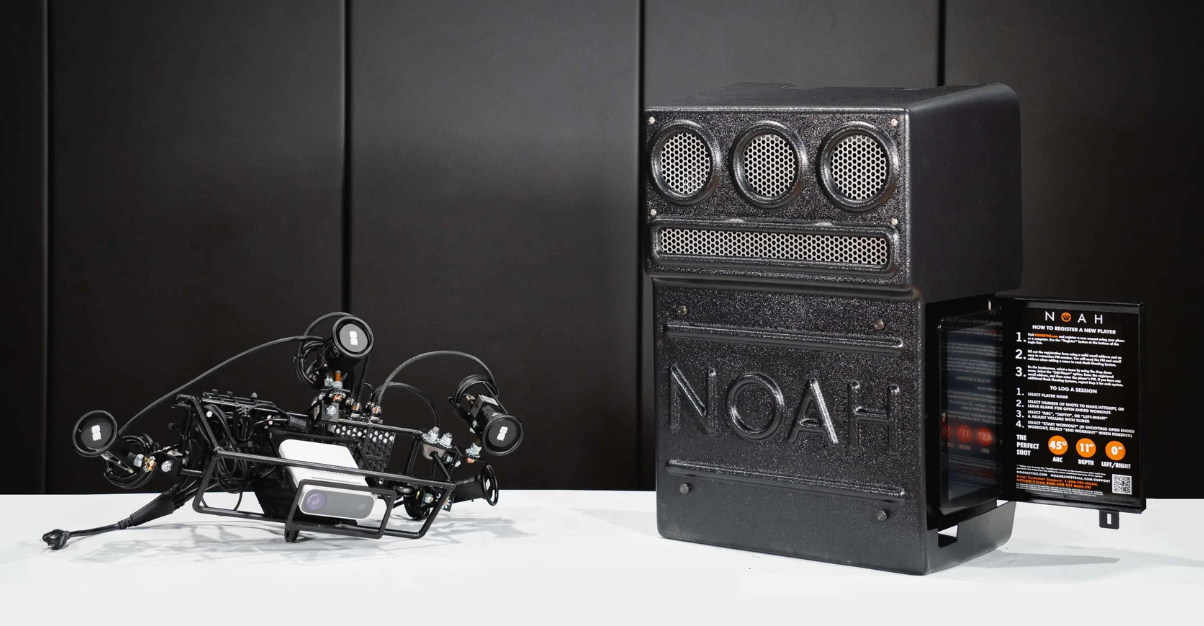
\includegraphics[width=0.75\linewidth]{resources/floats/ilustracoes/noah.png}
    \end{flushleft}
    \addcontentsline{lof}{figure}{Ilustração X – Hardware usado para a captação de arremessos}
\end{figura}
\FloatBarrier

\begin{figura}{Aplicativo do Noah Basketball}{Noah Basketball (2025)}
    \begin{flushleft}
        \label{fig:noah-app}
        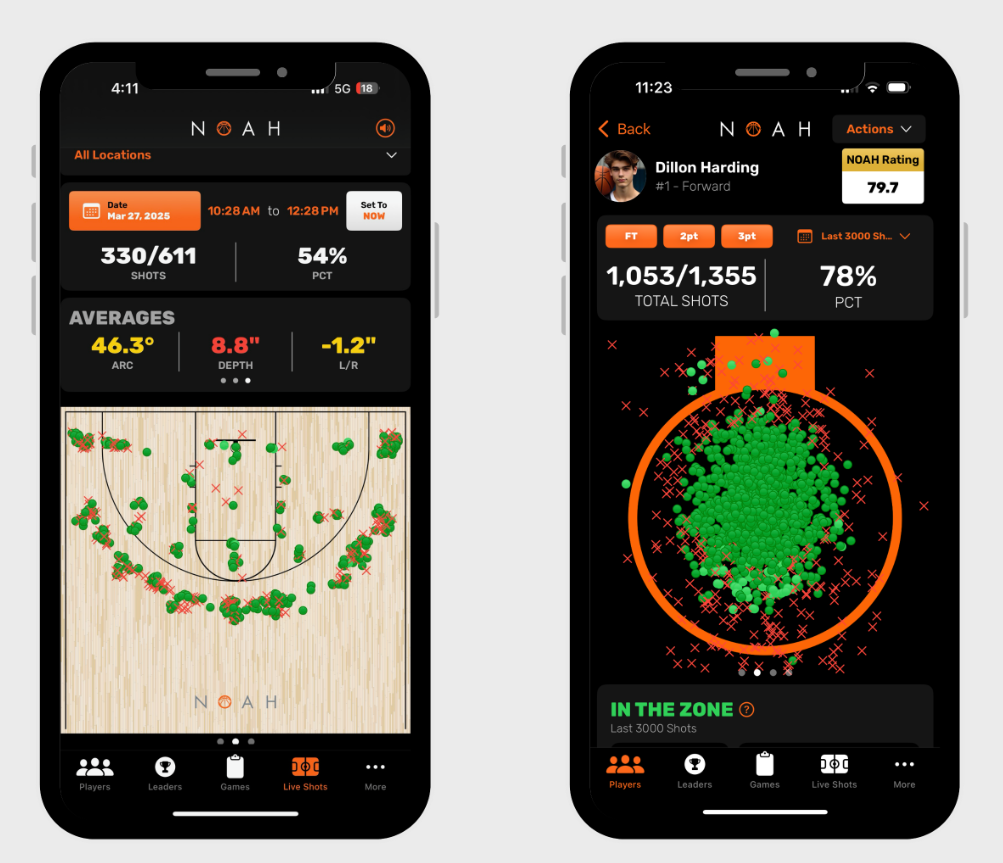
\includegraphics[width=0.65\linewidth]{resources/floats/ilustracoes/noahapp.png}
    \end{flushleft}
    \addcontentsline{lof}{figure}{Ilustração X – Aplicativo do Noah Basketball}
\end{figura}
\FloatBarrier

As ilustrações acima, em sequência, mostram o Hardware utilizado acima da tabela de basquete, que faz a captura dos arremessos, conseguindo assim por meio de \ac{cv} mapear o local exato do arremesso no aro. Com a captura dos arremessos,
é possível fazer a análise dos mesmos pelo aplicativo, podendo assim ver dados como porcentagem de acertividade e angulação média do arremesso.


\subsecao{Processamento de Imagens}

O processamento de imagens é um conjunto de técnicas aplicadas a imagens digitais com o objetivo de realçar características visuais, reduzir ruídos ou ajustar propriedades para facilitar a interpretação por sistemas computacionais. 
As operações típicas incluem nitidez, suavização, filtragem, binarização, realce de contraste e transformações geométricas.

Segundo a NVIDIA (2023), ``o processamento de imagens usa algoritmos para alterar imagens, incluindo nitidez, suavização, filtragem ou aprimoramento''. 
Já a \ac{cv}, por outro lado, ``não altera uma imagem, mas dá sentido ao que vê e realiza tarefas, como a rotulagem''. A empresa ainda destaca que o processamento de imagem pode ser usado como etapa preliminar, 
preparando a imagem para ser interpretada por modelos de \ac{cv}.

Em muitos sistemas modernos, especialmente os que utilizam \ac{cnn}, o pré-processamento da imagem é essencial para garantir que os dados visuais estejam padronizados e livres de ruídos que possam prejudicar o desempenho dos algoritmos. 
Ferramentas como \ac{opencv} e MATLAB são amplamente utilizadas nesse processo.

Dentre as principais técnicas aplicadas no processamento de imagens, destaca-se a \textbf{equalização de histograma}, que visa melhorar o contraste das imagens, 
redistribuindo os níveis de intensidade dos pixels e tornando as características visuais mais perceptíveis para os algoritlogos de detecção (OpenCV, 2025). 
Essa técnica é especialmente útil em ambientes com iluminação desigual, como ginásios esportivos, que é o caso deste trabalho.

Outra abordagem adotada é a \textbf{suavização da imagem}, geralmente feita com filtros como o \textit{Gaussian Blur}, 
que reduz ruídos de alta frequência e variações bruscas de cor que podem interferir na segmentação do corpo do atleta (OpenCV, 2025). 
Essa técnica atua como um pré-filtro, garantindo que a entrada da rede neural (\ac{yolo}) esteja mais limpa e menos sujeita a falsos positivos.

Além disso, é aplicada a \textbf{normalização de brilho e contraste}, por meio de transformações lineares na intensidade dos pixels, com o objetivo de uniformizar a exposição da imagem, 
garantindo consistência entre diferentes vídeos analisados (OpenCV, 2025). Isso contribui para a padronização das amostras de entrada.

\begin{figura}{Correção de contraste com OpenCV}{OpenCV (2025)}
    \begin{flushleft}
        \label{fig:contraste-opencv}
        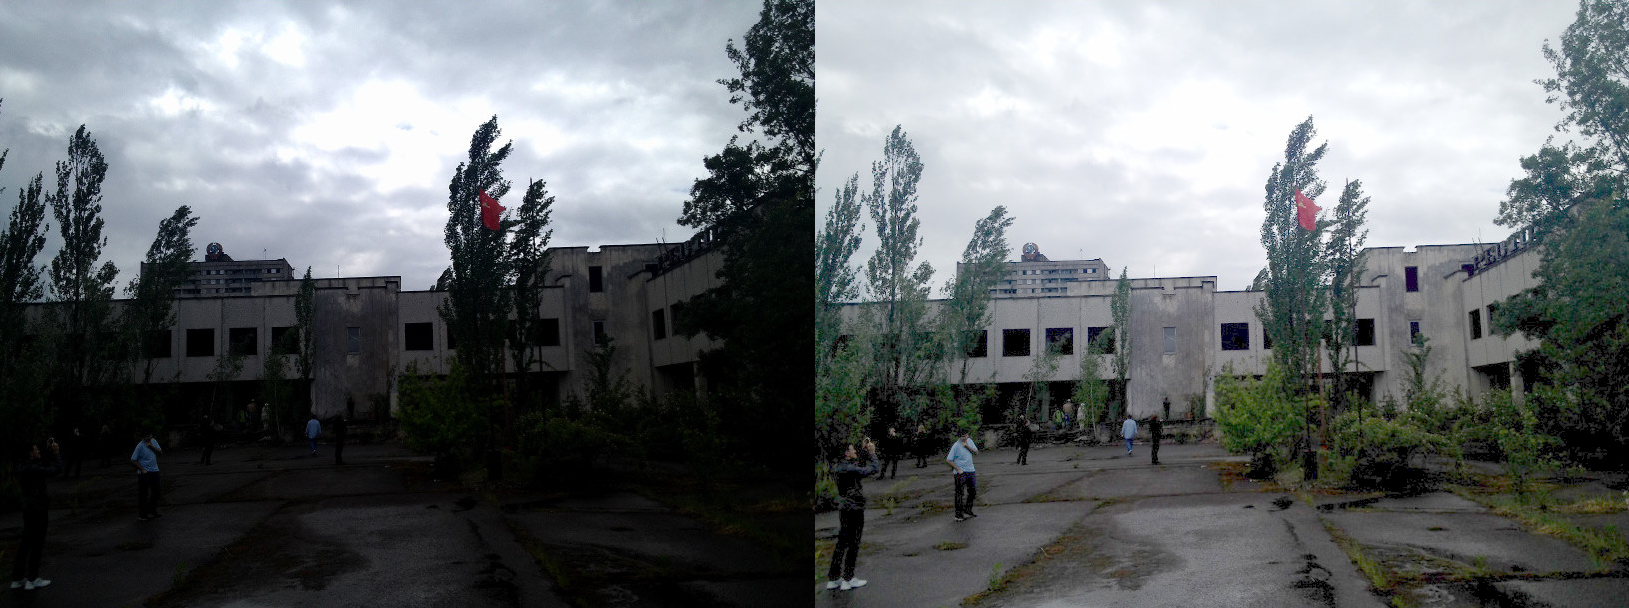
\includegraphics[width=0.85\linewidth]{resources/floats/ilustracoes/contraste.png}
    \end{flushleft}
    \addcontentsline{lof}{figure}{Ilustração X – Correção de contraste com OpenCV}
\end{figura}
\FloatBarrier

Esses procedimentos são executados em sequência como parte do \textbf{pipeline de pré-processamento}, visando fornecer imagens ideais para os modelos de \ac{cv} e posterior extração de características biomecânicas. 
Ferramentas como a biblioteca \ac{opencv} são utilizadas amplamente para essas finalidades, dada sua robustez e variedade de algoritmos implementados (OpenCV, 2025).


\secao{Modelos de Detecção de Poses e Estrutura Corporal}

A detecção de poses humanas é uma área da \ac{cv} voltada à identificação automática das articulações corporais em imagens ou vídeos. 
Através dessa tecnologia, é possível gerar uma estrutura esquelética baseada em pontos-chave (\textit{keypoints}), que permite a análise precisa de postura, movimentação e biomecânica do corpo (VISO.AI, 2023).

Segundo Boesch (2023), a tarefa de estimativa de pose pode ser classificada em dois grupos principais: detecção em 2D, que localiza as articulações no plano da imagem, e detecção em 3D, que busca reconstruir a estrutura corporal tridimensional. 
Embora a detecção em 3D ofereça maior contexto espacial, a abordagem 2D permanece amplamente utilizada devido à sua eficiência e maior disponibilidade de \textit{datasets} anotados.

Entre os principais modelos atuais, destacam-se:

\begin{myitemize}
    \item \textbf{OpenPose}: Um dos primeiros frameworks de código aberto capazes de detectar múltiplas pessoas em tempo real, mapeando pontos da face, mãos e corpo de forma simultânea. 
    Utiliza uma abordagem \textit{bottom-up}, identificando os pontos-chave primeiro para depois agrupá-los por indivíduo (Boesch, 2023; PAPERSWITHCODE, 2024).
    
    \item \textbf{BlazePose}: Criado pelo Google, é um modelo otimizado para dispositivos móveis. Utiliza uma malha corporal com 33 pontos e apresenta excelente desempenho em aplicações que requerem baixa latência, 
    como jogos e aplicativos de condicionamento físico (AIP PUBLISHING, 2023).
    
    \item \textbf{PoseNet}: Também desenvolvido pelo Google, é amplamente usado por sua leveza e por funcionar diretamente em navegadores com imagens RGB, o que o torna prático para aplicações web e mobile (CODERADE.IO, 2024).
\end{myitemize}

Esses modelos têm sido empregados na realidade aumentada, fisioterapia digital e na análise esportiva, permitindo monitoramento técnico em multiplos esportes, tanto coletivos quanto individuais com uso de câmeras comuns.
Abaixo, por meio de uma tabela, serão abordados os principais aspectos desses modelos.

\vspace{0.5cm}
    \begin{tabela}{Comparação entre modelos de detecção de pose corporal}{O Autor, adaptado de Boesch (2023), PapersWithCode (2024), AI Publishing (2023) e Coderade.io (2024)}
        \label{tab:poses}
        \resizebox{0.8\textwidth}{!}{ % Redimensiona a tabela para caber na largura da página
        \begin{tabularx}{\textwidth}{|X|X|X|X|}
            \hline
            \textbf{Critério} & \textbf{OpenPose} & \textbf{BlazePose} & \textbf{PoseNet} \\ \hline
            \textbf{Desenvolvedor} & Carnegie Mellon University & Google & Google \\ \hline
            \textbf{Número de pontos detectados} & Variável (face, mãos e corpo completo) & 33 pontos corporais & 17 pontos corporais \\ \hline
            \textbf{Abordagem técnica} & Bottom-up & Top-down & Top-down \\ \hline
            \textbf{Aplicações principais} & Detecção múltipla simultânea, análise detalhada de movimentos & Jogos, aplicativos móveis e condicionamento físico & Aplicações leves em navegadores e dispositivos móveis \\ \hline
            \textbf{Precisão e desempenho} & Alta precisão, maior consumo computacional & Alta precisão, otimizado para baixa latência & Precisão moderada, desempenho otimizado \\ \hline
            \textbf{Ambientes de uso} & Ambientes controlados e pesquisa avançada & Aplicações móveis e interativas & Aplicações web e mobile leves \\ \hline
            \textbf{Disponibilidade e popularidade} & Alta (open source) & Alta (amplamente usado) & Alta (amplamente usado) \\ \hline
        \end{tabularx}}
    \end{tabela}

\vspace{0.5cm}


\secao{Redes Neurais Convolucionais}

As redes neurais convolucionais (CNNs) surgiram como uma poderosa arquitetura dentro do campo de aprendizado profundo, especialmente eficazes para o reconhecimento de padrões em imagens, vídeos e dados com estrutura espacial. 
Ao contrário das redes totalmente conectadas (MLPs), as \acp{cnn} exploram o princípio da localidade espacial e da invariância translacional, o que permite reduzir drasticamente a quantidade de parâmetros e melhorar a generalização dos modelos. 
Isso é possível graças à aplicação de filtros convolucionais que percorrem localmente a entrada, extraindo características relevantes em diferentes escalas e posições (GOODFELLOW; BENGIO; COURVILLE, 2016).

Essas redes são compostas, em sua forma mais básica, por camadas convolucionais, funções de ativação (como ReLU), camadas de pooling (que reduzem a dimensionalidade), e camadas totalmente conectadas ao final do modelo para classificação ou regressão. 
Em contextos visuais, por exemplo, as primeiras camadas de uma \ac{cnn} aprendem a detectar bordas e texturas simples, enquanto camadas mais profundas passam a identificar formas e padrões mais complexos, 
como olhos ou rostos em imagens humanas (ARORA et al., 2021).

A capacidade hierárquica de representação é uma das grandes forças das \acp{cnn}. Como mencionado por Arora et al. (2021), os filtros nas primeiras camadas capturam características de baixo nível (e.g., bordas), 
enquanto as camadas subsequentes combinam essas informações para formar representações mais abstratas. O processo de aprendizado ocorre por meio da retropropagação (backpropagation), 
otimizando os pesos dos filtros conforme os erros na saída do modelo (KARPATHY; LI, 2023).

Além disso, a natureza parametrizada dos filtros permite que uma \ac{cnn} reconheça um objeto independentemente da sua posição na imagem, promovendo o conceito de invariância espacial, 
essencial em aplicações como reconhecimento facial, classificação de imagens médicas e detecção de objetos.

\subsecao{YOLO (You Only Look Once)}

YOLO (\textit{You Only Look Once}) é uma arquitetura de rede neural para detecção de objetos em tempo real, proposta por Redmon et al. (2016). 
Ao contrário de abordagens tradicionais como R-CNN, que realizam múltiplos estágios no processo de detecção, \ac{yolo} reformula o problema como uma única tarefa de regressão, mapeando diretamente a imagem para caixas delimitadoras e probabilidades de classe. 
Segundo os autores, ``reformulamos a detecção de objetos como um problema de regressão única, direto dos pixels da imagem para as coordenadas das caixas e as probabilidades das classes'' (REDMON et al., 2016).

A estrutura da rede divide a imagem de entrada em uma grade (geralmente 7×7). Cada célula da grade é responsável por prever um número fixo de \textit{bounding boxes} e suas respectivas pontuações de confiança, além da classificação dos objetos presentes. 
A arquitetura original da \ac{yolo} é composta por 24 camadas convolucionais e duas totalmente conectadas, utilizando a rede \textit{Darknet} como base (CARVALHO et al., 2022).

O guia técnico da Encord (2024) destaca que ``a \ac{yolo} processa a imagem inteira de uma vez, permitindo que a rede aprenda representações contextuais mais globais e reduza erros comuns, como falsas detecções em regiões de fundo''. 
Essa abordagem global é uma das principais vantagens da \ac{yolo} em relação a métodos que se concentram apenas em regiões localizadas da imagem.

Nos testes realizados pelos autores originais, o modelo atingiu desempenho superior a 45 \ac{fps} com latência inferior a 25 milissegundos, possibilitando aplicações em vídeo em tempo real (REDMON et al., 2016).

Além disso, Carvalho et al. (2022) explicam que a \ac{yolo} combina os dois processos fundamentais da detecção de objetos — classificação e localização — em uma única etapa, tornando o processo mais eficiente. 
Eles afirmam que ``\ac{yolo} é capaz de responder duas perguntas: quais objetos estão na imagem? E onde eles estão posicionados?'' (CARVALHO et al., 2022).

\begin{figura}{Uso da YOLO em partidas da NBA}{FRANCI, Simone, (2024)}
    \begin{flushleft}
        \label{fig:NBA}
        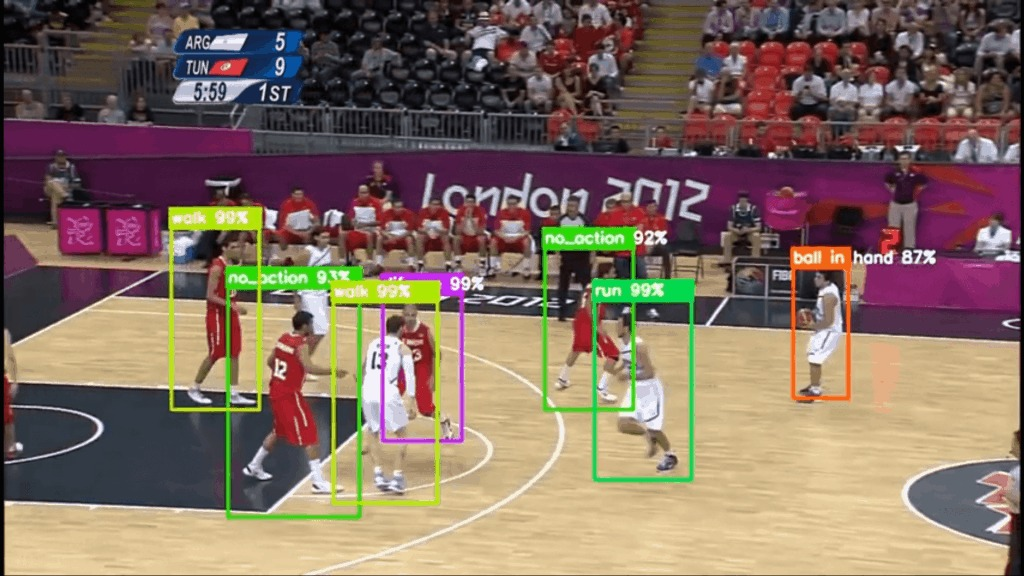
\includegraphics[width=0.7\linewidth]{resources/floats/ilustracoes/NBA.jpg}
    \end{flushleft}
    \addcontentsline{lof}{figure}{Ilustração X – Uso da visão computacional em partidas da NBA}
\end{figura}
\FloatBarrier

% --- Início da Seção de Evolução e Comparação (CONTEÚDO NOVO) ---

\subsubsecao{Evolução das Versões do YOLO}

Desde sua criação, o framework \ac{yolo} evoluiu significativamente, com novas versões que aprimoraram a velocidade, a precisão e a versatilidade. 
As versões desenvolvidas pela Ultralytics mais conhecidas são \textbf{YOLOv5}, \textbf{YOLOv8}, e a iteração estável mais recente, o \textbf{YOLOv11}. 
O YOLOv8 expandiu o framework para incluir nativamente múltiplas tarefas, como a estimação de pose, enquanto o YOLOv11 focou em otimizar a eficiência, buscando maior precisão com um menor número de parâmetros que seu antecessor (Ultralytics, 2024).

A tabela 2 a seguir compara as três principais versões do \ac{yolo}, com informações retiradas do site do desenvolvedor:

\vspace{0.5cm}
\begin{tabela}{Comparativo entre as Principais Versões do YOLO (Ultralytics).}{O Autor, adaptado de Ultralytics (2024)}
    \label{tab:yolo-comparativo}
    \resizebox{1.0\textwidth}{!}{
    \begin{tabular}{|x|x|x|x|} % Usando colunas 'l' e 'c' como no seu último exemplo
        \hline
        \textbf{Característica} & \textbf{YOLOv5} & \textbf{YOLOv8} & \textbf{YOLOv11} \\
        \hline
        Arquitetura (Head) & \begin{tabular}[x]{@{}x@{}}Baseada em Âncoras \\ (Anchor-Based)\end{tabular} & \begin{tabular}[x]{@{}x@{}}Livre de Âncoras \\ (Anchor-Free)\end{tabular} & \begin{tabular}[x]{@{}x@{}}Mantém a abordagem Livre de \\ Âncoras com backbone e \\ neck aprimorados.\end{tabular} \\
        \hline
        Tarefas Suportadas & \begin{tabular}[x]{@{}x@{}}Foco principal em \\ Detecção de Objetos.\end{tabular} & \begin{tabular}[x]{@{}x@{}}Suporte nativo a Detecção, \\ Segmentação, Estimação de Pose, \\ Rastreamento e Classificação.\end{tabular} & \begin{tabular}[x]{@{}x@{}}Mantém e aprimora a gama \\ de tarefas do YOLOv8, incluindo \\ Detecção Orientada (OBB).\end{tabular} \\
        \hline
        Principal Avanço & \begin{tabular}[x]{@{}x@{}}Popularização do balanço \\ entre alta velocidade \\ e boa precisão.\end{tabular} & \begin{tabular}[x]{@{}x@{}}Introdução de um framework \\ multitarefa com API unificada e \\ modelos pré-treinados.\end{tabular} & \begin{tabular}[x]{@{}x@{}}Foco em eficiência computacional: \\ alcançar maior precisão com \\ menos parâmetros que o YOLOv8.\end{tabular} \\
        \hline
        Modelo para Pose & \begin{tabular}[x]{@{}x@{}}Não possui um modelo \\ oficial na versão original.\end{tabular} & \begin{tabular}[x]{@{}x@{}}Inclui modelos \\ \textbf{YOLOv8-Pose} pré-treinados \\ e prontos para uso.\end{tabular} & \begin{tabular}[x]{@{}x@{}}Inclui modelos \\ \textbf{YOLOv11-Pose} pré-treinados, \\ continuando o suporte \\ nativo à tarefa.\end{tabular} \\
        \hline
    \end{tabular}
    } % Fim do resizebox
\end{tabela}
\vspace{0.5cm}

A arquitetura do YOLOv8, ilustrada de forma simplificada na figura, é a base para o seu alto desempenho e pode ser dividida em três componentes principais que segundo Ultralytics (2025) são:

\begin{itemize}
    \item \textbf{Backbone (Coluna Vertebral):} É a primeira parte da rede, responsável por extrair características importantes da imagem de entrada. 
    Ele processa a imagem em várias camadas (P1 a P5), onde a resolução espacial diminui, mas a complexidade semântica da informação aumenta. Características de diferentes níveis (P3, P4, P5) são então enviadas para a próxima etapa.

    \item \textbf{Neck (Pescoço):} Atua como uma ponte, mesclando e combinando as características que vêm do \textit{Backbone}. 
    Utilizando uma estrutura de Agregação de Caminho (Path Aggregation Network - PANet), ele funde a informação semântica das camadas profundas (que sabem ``o que'' é um objeto) 
    com a informação espacial das camadas mais rasas (que sabem exatamente ``onde'' ele está). Isso é fundamental para detectar objetos de diferentes tamanhos.

    \item \textbf{Head (Cabeça):} É a parte final, responsável por realizar as predições. Ela recebe os mapas de características refinados do \textit{Neck} e utiliza múltiplas ``cabeças de detecção'', 
    cada uma especializada em uma escala (objetos pequenos, médios e grandes). A saída final são as caixas delimitadoras, a classe e a confiança de cada objeto detectado — ou, no caso do YOLO-Pose, as coordenadas dos keypoints.
\end{itemize}

\begin{figura}{Arquitetura da YOLOv8 simplificada}{Jocher et al. (2023)}
    \begin{flushleft}
        \label{fig:arqyolo}
        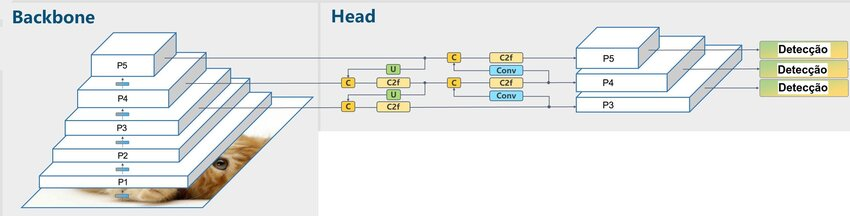
\includegraphics[width=1.0\linewidth]{resources/floats/ilustracoes/arquiteturayolo.png}
    \end{flushleft}
    \addcontentsline{lof}{figure}{Ilustração X – Arquitetura da YOLOv8 simplificada}
\end{figura}
\FloatBarrier

\subsubsecao{YOLO-Pose para Análise de Keypoints}

Para a análise biomecânica de arremessos, que depende da identificação precisa de articulações, as variantes de estimação de pose do \ac{yolo} são as ferramentas mais adequadas. 
Tanto o \textbf{YOLOv8-Pose} quanto o \textbf{YOLOv11-Pose} são modelos construídos para, além de localizar uma pessoa na imagem, estimar a posição de seus \textbf{17 keypoints corporais} (Ultralytics, 2024).

Esses pontos-chave, treinados no dataset COCO-pose, incluem as principais articulações para a análise de movimento, como ombros, cotovelos, punhos, quadris, joelhos e tornozelos. 
A saída do modelo fornece as coordenadas (x, y) e um score de confiança para cada keypoint detectado, permitindo a construção de um esqueleto digital do atleta para posterior cálculo de ângulos e trajetórias. 

A escolha entre os diferentes tamanhos de modelos disponíveis (nano, small, medium, etc.) é uma decisão fundamental do projeto, permitindo um balanço entre a velocidade de inferência e a precisão da detecção, 
um fator crucial a ser definido dependendo dos requisitos computacionais do hardware disponível, como uma \ac{gpu} NVIDIA. (Ultralytics, 2024).

\secao{Python e suas Bibliotecas para Visão Computacional}

Python é uma linguagem de programação de alto nível que tem se consolidado como uma das principais ferramentas para o desenvolvimento de aplicações em ciência de dados, \ac{ml} e \ac{cv}. 
Sua popularidade se deve à sintaxe simples, à extensa comunidade ativa e à ampla variedade de bibliotecas disponíveis, que facilitam o desenvolvimento de projetos robustos com pouco código. 
Paiva et al. (2019) destacam que Python é uma linguagem ideal para iniciantes por sua simplicidade e clareza, mas que também oferece poderosas funcionalidades utilizadas em ambientes acadêmicos e industriais.

No campo da \ac{cv}, destaca-se a biblioteca \ac{opencv}, que fornece algoritmos eficientes para captura, manipulação e análise de imagens e vídeos. Como apontado por Antonello (2016), 
o \ac{opencv} permite realizar desde operações básicas, como redimensionamento e suavização, até tarefas mais avançadas, como detecção de objetos, segmentação e rastreamento em tempo real. 
A biblioteca é complementada pelo uso de ferramentas como NumPy, essencial para operações com matrizes, e Matplotlib, que auxilia na visualização e interpretação gráfica dos dados (Data Hackers, 2019).

\begin{figura}{Uso da biblioteca OpenCV e Matplotlib no Google Colab}{O Autor}
    \begin{flushleft}
        \label{fig:opencv-colab}
        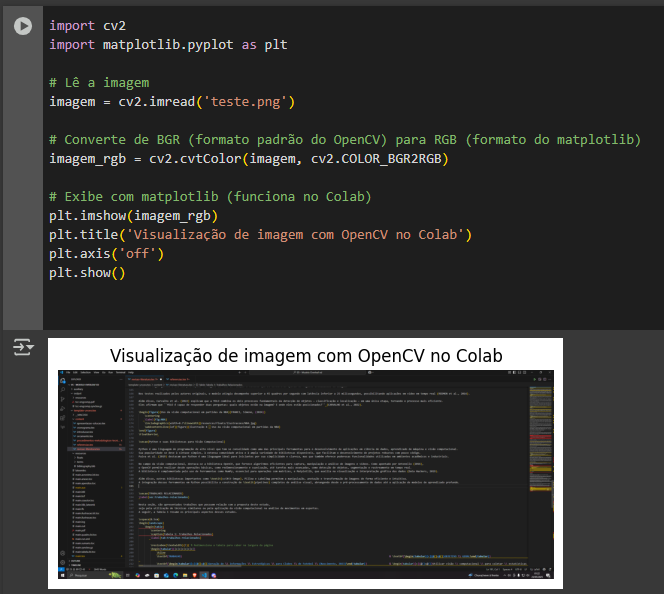
\includegraphics[width=0.60\linewidth]{resources/floats/ilustracoes/opencv.png}
    \end{flushleft}
    \addcontentsline{lof}{figure}{Ilustração X – Uso da biblioteca OpenCV e Matplotlib no Google Colab}
\end{figura}
\FloatBarrier

\begin{figura}{Uso da biblioteca Matplotlib}{O Autor}
    \begin{flushleft}
        \label{fig:matplotlib-exemplo}
        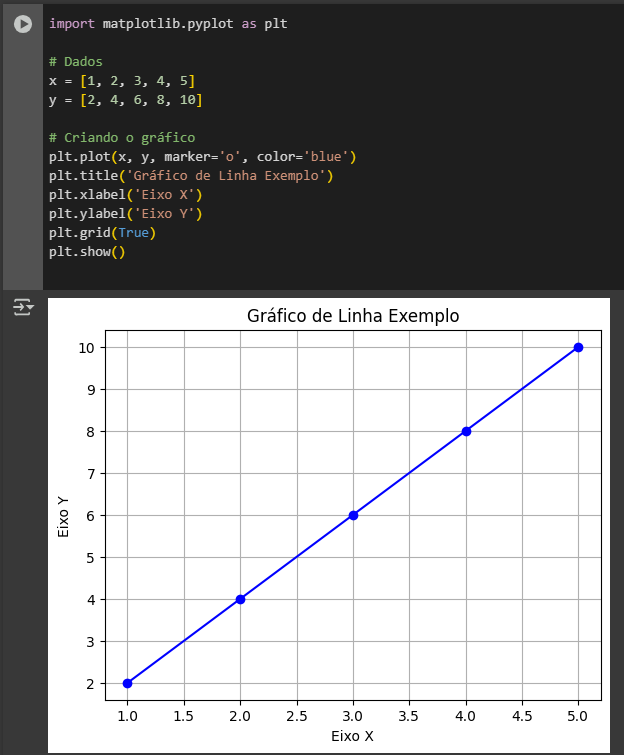
\includegraphics[width=0.48\linewidth]{resources/floats/ilustracoes/matplotlib.png}
    \end{flushleft}
    \addcontentsline{lof}{figure}{Ilustração X – Uso da biblioteca Matplotlib}
\end{figura}
\FloatBarrier

Além disso, outras bibliotecas importantes como \textit{scikit-image}, Pillow e LabelImg permitem a manipulação, anotação e transformação de imagens de forma eficiente e intuitiva. 
A integração dessas ferramentas em Python possibilita a construção de \textit{pipelines} completos de análise visual, abrangendo desde o pré-processamento de dados até a aplicação de modelos de aprendizado profundo.

\secao{TRABALHOS RELACIONADOS}
\label{sec:trabalhos-relacionados}

Nesta seção, são apresentados trabalhos que possuem relação com a proposta deste estudo, 
seja pela utilização de técnicas similares ou pela aplicação da \ac{cv} na análise de movimentos em esportes. A seguir, cada um dos trabalhos é abordado individualmente, seguido de uma tabela comparativa ao final.

\subsecao{Geração de Informações Estratégicas para Clubes de Futebol (Nascimento, 2023)}

O trabalho de Nascimento (2023) propõe um sistema de \ac{cv} que utiliza o algoritmo \ac{yolo} para detectar jogadores e rastrear a trajetória da bola em partidas de futebol. 
O objetivo principal é fornecer estatísticas estratégicas, como contagem de passes e ocupação espacial, auxiliando a comissão técnica durante análises táticas.

A arquitetura do sistema inclui módulos de detecção, rastreamento e análise. Os testes realizados mostraram precisão variando entre 40\% e 90\% na contagem de passes, com bons níveis de eficiência na trajetória da bola.

\begin{figura}{Detecção de jogadores em campo utilizando YOLO}{Nascimento, 2023}
    \begin{flushleft}
        \label{fig:Futebol}
        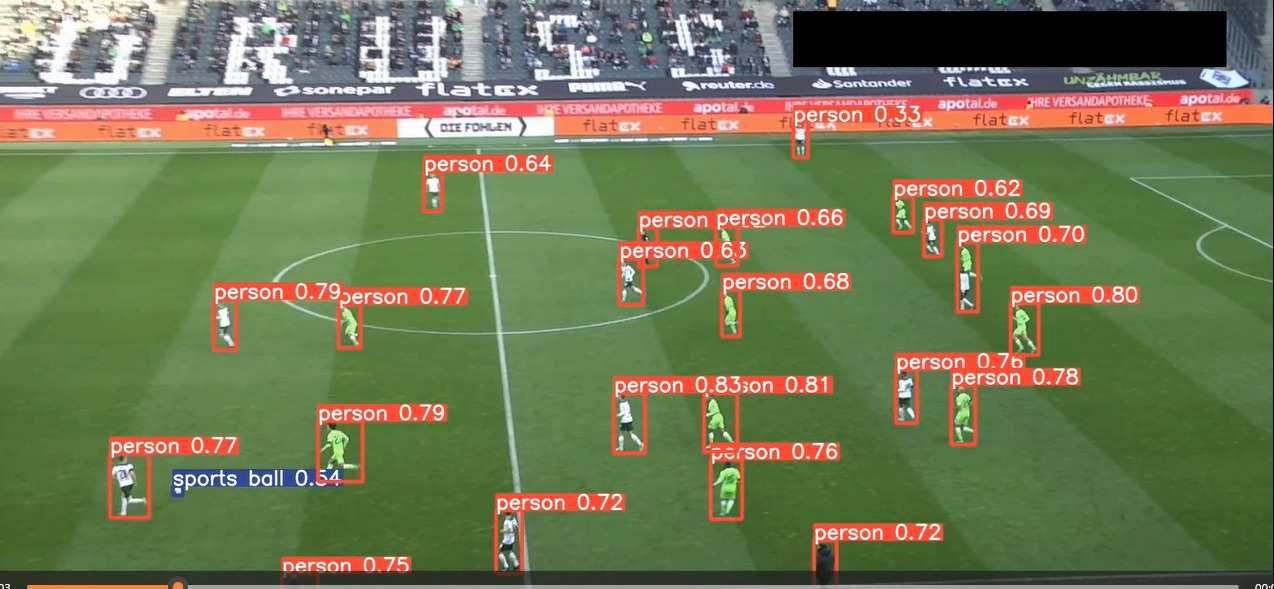
\includegraphics[width=0.48\linewidth]{resources/floats/ilustracoes/FUTEBOL.jpg}
    \end{flushleft}
    \addcontentsline{lof}{figure}{Ilustração X – Detecção de jogadores em campo utilizando YOLO}
\end{figura}
\FloatBarrier

\subsecao{Classificação de Golpes de Karate (Teixeira, 2024)}

Teixeira (2024) desenvolveu um sistema de reconhecimento de ações voltado à classificação de golpes de Karate. O sistema emprega a detecção de \textit{keypoints} corporais com base em \ac{cv}, 
utilizando as bibliotecas OpenPose, YOLOv5 e algoritmos de classificação como SVM.

Os dados capturados durante os movimentos são processados em tempo real para identificar padrões específicos de golpes. Os testes apontaram precisão de 99,45\% e latência de processamento adequada para aplicações em treinamento e arbitragem automatizada.

\begin{figura}{Detecção de \textit{keypoints} durante execução de golpes}{Teixeira, 2024}
    \begin{flushleft}
        \label{fig:keypoints}
        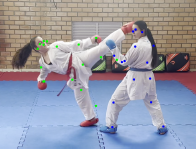
\includegraphics[width=0.36\linewidth]{resources/floats/ilustracoes/KEYPOINTS.png}
    \end{flushleft}
    \addcontentsline{lof}{figure}{Ilustração X – Detecção de \textit{keypoints} durante execução de golpes}
\end{figura}
\FloatBarrier

\subsecao{Biomechanical Analysis of Shooting Performance (Pan et al., 2021)}

O estudo de Pan et al. (2021) investigou o desempenho de arremessos no basquetebol por meio de uma análise biomecânica baseada em \ac{cv}. 
O sistema faz uso de sensores Kinect Azure para capturar o movimento dos atletas e aplica modelos de esqueleto para medir postura, ângulo de lançamento e tempo de execução.

O objetivo da pesquisa foi entender como fatores como postura corporal e coordenação influenciam a precisão do arremesso. 
Os resultados mostraram que diferenças significativas entre gêneros foram observadas e que a postura está diretamente ligada ao desempenho.

\begin{figura}{Modelo esquelético utilizado para análise biomecânica}{Pan et al., 2022}
    \begin{flushleft}
        \label{fig:esqueleto}
        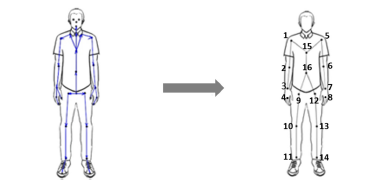
\includegraphics[width=0.48\linewidth]{resources/floats/ilustracoes/ESQUELETO.png}
    \end{flushleft}
    \addcontentsline{lof}{figure}{Ilustração X – Modelo esquelético utilizado para análise biomecânica}
\end{figura}
\FloatBarrier

Ao final dessa seção, a Tabela 3 resume os principais aspectos desses estudos abordados.

Ambos os estudos demonstram que a \ac{cv} pode ser aplicada com sucesso na análise esportiva, 
reforçando a viabilidade do presente trabalho e oferecendo referências metodológicas para a implementação e validação do sistema de análise de arremesso no basquete.


    \begin{tabela}{Trabalhos Relacionados}{O Autor}
        \label{tab:trabalhos-relacionados}
        \resizebox{\textwidth}{!}{ % Redimensiona a tabela para caber na largura da página
        \begin{tabular}{|c|c|c|c|c|c|}
            \hline
            \textbf{TRABALHO}                                                                                                                                           & \textbf{\begin{tabular}[c]{@{}c@{}}OBJETIVO \\ GERAL\end{tabular}}                                                                                                                           & \textbf{TECNOLOGIAS}                                                                                                                                      & \textbf{\begin{tabular}[c]{@{}c@{}}MÉTRICAS E \\ VALIDAÇÃO\end{tabular}}                                                                                           & \textbf{\begin{tabular}[c]{@{}c@{}}QUESTÃO \\ DE PESQUISA\end{tabular}}                                                                                & \textbf{\begin{tabular}[c]{@{}c@{}}RESULTADOS \\ ALCANÇADOS\end{tabular}}                                                                         \\ \hline

            \textbf{\begin{tabular}[c]{@{}c@{}}Geração de \\ Informações \\ Estratégicas \\ para Clubes \\ de Futebol \\ (Nascimento, 2023)\end{tabular}}               & \begin{tabular}[c]{@{}c@{}}Utilizar visão \\ computacional \\ para coletar \\ estatísticas em \\ partidas de \\ futebol, como \\ contagem de \\ passes e trajetória \\ da bola.\end{tabular} & \begin{tabular}[c]{@{}c@{}}YOLO para \\ detecção de \\ jogadores e \\ rastreamento da \\ bola; Redes \\ Neurais \\ Convolucionais \\ (CNNs).\end{tabular} & \begin{tabular}[c]{@{}c@{}}Precisão \\ variando entre \\ 40\% e 90\% \\ para contagem \\ de passes; \\ Eficiência \\ na trajetória \\ da bola.\end{tabular}        & \begin{tabular}[c]{@{}c@{}}Como aplicar \\ visão \\ computacional \\ para coletar \\ estatísticas de \\ futebol de \\ forma precisa?\end{tabular}      & \begin{tabular}[c]{@{}c@{}}Implementação \\ bem-sucedida \\ da tecnologia, \\ com impacto \\ na análise tática.\end{tabular}                      \\ \hline

            \textbf{\begin{tabular}[c]{@{}c@{}}Classificação \\ de Golpes de \\ Karate \\ (Teixeira, 2024)\end{tabular}}                                                & \begin{tabular}[c]{@{}c@{}}Utilizar visão \\ computacional \\ para classificar \\ golpes de Karate e \\ auxiliar na \\ arbitragem e \\ treinamento.\end{tabular}                             & \begin{tabular}[c]{@{}c@{}}YOLO para \\ detecção de \\ keypoints; \\ Redes Neurais \\ Convolucionais \\ (CNNs); \\ Algoritimo \\ SVM.\end{tabular}        & \begin{tabular}[c]{@{}c@{}}FPS e latência \\ por quadro \\ como métricas;\\ Precisão de \\ 99,45\% no \\ recebimento \\ de golpes.\end{tabular}                    & \begin{tabular}[c]{@{}c@{}}Como aplicar \\ aprendizado de \\ máquina \\ para reconhecimento \\ e classificação \\ de golpes \\ no Karate?\end{tabular} & \begin{tabular}[c]{@{}c@{}}Modelo \\ eficiente para \\ análise de golpes, \\ útil para \\ arbitragem \\ automatizada.\end{tabular}                \\ \hline

            \textbf{\begin{tabular}[c]{@{}c@{}}Biomechanical \\ Analysis of \\ Shooting \\ Performance \\ for Basketball \\ Players (Pan \\ et al., 2021)\end{tabular}} & \begin{tabular}[c]{@{}c@{}}Analisar \\ biomecanicamente \\ o desempenho de \\ arremesso no \\ basquetebol com \\ visão \\ computacional.\end{tabular}                                        & \begin{tabular}[c]{@{}c@{}}Kinect Azure \\ para captura \\ de movimento; \\ Processamento \\ de dados \\ cinemáticos.\end{tabular}                        & \begin{tabular}[c]{@{}c@{}}Análise \\ estatística das \\ diferenças \\ entre gêneros \\ no arremesso; \\ Correlação \\ entre postura \\ e eficiência.\end{tabular} & \begin{tabular}[c]{@{}c@{}}Como a \\ visão \\ computacional \\ pode contribuir \\ para a análise \\ biomecânica \\ do arremesso?\end{tabular}          & \begin{tabular}[c]{@{}c@{}}Resultados \\ mostraram que a \\ coordenação \\ e a postura \\ influenciam a \\ precisão do \\ arremesso.\end{tabular} \\ \hline

        \end{tabular}}

    \end{tabela}

\vspace{0.5 cm}

As pesquisas bibliográficas a seguir foram feitas dentro do Google Acadêmico em Março de 2025, 
a plataforma Sci-Hub também foi utilizada para procurar artigos que são pagos na plataforma do Google, 
porém não foram encontradas amostras na plataforma. Na tabela 4, podemos ver detalhes de resultados obtidos nas pesquisas avançadas de trabalhos relacionados, 
todos os termos foram pesquisados utilizando como pesquisa palavras utilizadas no título de artigos, trabalhos que utilizam a visão computacional tiveram um maior número de resultados, já trabalhos com o tema \ac{yolo} em específico foram mais difíceis de se encontrar.

\begin{tabela}{Resultados das pesquisas por termos no título de artigos}{O Autor}
\label{tab:resultados-pesquisa}
\begin{tabular}{|c|c|c|}
\hline
\textbf{Termos Pesquisados} & \textbf{Período de Tempo} & \textbf{Resultados Obtidos} \\
\hline
Visão computacional, esporte, yolo & 2005 - 2025 & 50 resultados \\
Basquete, visão computacional       & 2005 - 2025 & Nenhum resultado \\
Yolo, esporte                       & 2005 - 2025 & Nenhum resultado \\
Yolo, sports                        & 2005 - 2025 & 7 resultados \\
Computer vision, basketball         & 2005 - 2025 & 22 resultados \\
\hline
\end{tabular}
\end{tabela}
\vspace{0.5cm}



